\documentclass{article}
\usepackage[margin=1in]{geometry}
\usepackage{amsmath,amsthm,amssymb}
\usepackage{bbm,enumerate,mathtools}
\usepackage{tikz,pgfplots}
\usepackage{chessboard}
\usepackage[hidelinks]{hyperref}
\usepackage{multicol} % Problem 35
\usepackage{xstring} % Difficulty command
\usetikzlibrary{shapes.geometric}

\newenvironment{question}{\begin{trivlist}\item[\textbf{Question.}]}{\end{trivlist}}
\newenvironment{note}{\begin{trivlist}\item[\textbf{Note.}]}{\end{trivlist}}
\newenvironment{references}{\begin{trivlist}\item[\textbf{References.}]}{\end{trivlist}}
\newenvironment{related}{\begin{trivlist}\item[\textbf{Related.}]\end{trivlist}\begin{enumerate}}{\end{enumerate}}

\newcommand\score[1]{
\pgfmathsetmacro\pgfxa{#1+1}
\tikzstyle{scorestars}=[
  star,
  star points=5,
  star point ratio=2.25,
  draw,
  inner sep=3pt,
  anchor=outer point 5
]
  \begin{tikzpicture}[baseline]
    \draw[opacity=0] (0,-0.5) rectangle (0,0.2); % Workaround for whitespace at the bottom.
    \foreach \i in {1,...,4} {
      \pgfmathparse{(\i<=#1?"yellow":"gray")}
      \edef\starcolor{\pgfmathresult}
      \draw (\i*4.5ex,0) node[name=star\i,scorestars,fill=\starcolor]  {};
    }
  \end{tikzpicture}
}

\newcommand{\difficulty}[1]{%
  \IfEqCase{#1}{%
      {1}{
        
\begin{tikzpicture}[scale=0.7, baseline=0.9mm]%
          \definecolor{slopegreen}{rgb}{0.0, 0.5, 0.0}%
          \fill[slopegreen] (0.5,0.5) circle (0.5);%
        \end{tikzpicture}%
      }%
      {2}{
        
\begin{tikzpicture}[scale=0.7, baseline=0.9mm]%
          \definecolor{slopeblue}{rgb}{0.0, 0.44, 1.00}
          \fill[slopeblue] (0,0) rectangle (1,1);%
        \end{tikzpicture}%
      }%
      {3}{
\begin{tikzpicture}[scale=0.7, baseline=0.9mm]\fill (0,0.5)--(0.5, 0)--(1,0.5)--(0.5,1)--cycle; \end{tikzpicture}}%
      {4}{
\begin{tikzpicture}[scale=0.7, baseline=0.9mm]\fill (0.25,0)--(0,0.5)--(0.25,1)--(0.5,0.5)--cycle; \fill (0.75,0)--(0.5,0.5)--(0.75,1)--(1,0.5)--cycle;\end{tikzpicture}}%
      % you can add more cases here as desired
  }[\PackageError{difficulty}{Undefined difficulty level: #1}{}]%
}%
\newcommand{\rating}[2]{\difficulty{#1}\\\score{#2}\\}


\begin{document}

\rating{3}{3}
Consider arrangements of $n$ lines in the plane.
\begin{figure}[ht!]
  \centering
  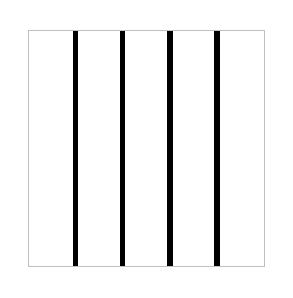
\begin{tikzpicture}[scale=3]
    \draw[line width=2] (0.2,0)--(0.2,1);
    \draw[line width=2] (0.4,0)--(0.4,1);
    \draw[line width=2] (0.6,0)--(0.6,1);
    \draw[line width=2] (0.8,0)--(0.8,1);
    \draw[gray!50] (0,0) rectangle (1, 1);
  \end{tikzpicture}
  ~
  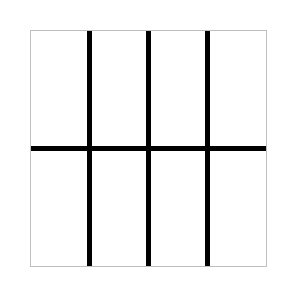
\begin{tikzpicture}[scale=3]
    \draw[line width=2] (0.25,0)--(0.25,1);
    \draw[line width=2] (0.5,0)--(0.5,1);
    \draw[line width=2] (0.75,0)--(0.75,1);
    \draw[line width=2] (0,0.5)--(1,0.5);
    \draw[gray!50] (0,0) rectangle (1, 1);
  \end{tikzpicture}
  ~
  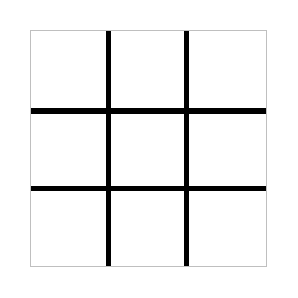
\begin{tikzpicture}[scale=3]
    \draw[line width=2] (0.33,0)--(0.33,1);
    \draw[line width=2] (0.66,0)--(0.66,1);
    \draw[line width=2] (0,0.33)--(1,0.33);
    \draw[line width=2] (0,0.66)--(1,0.66);
    \draw[gray!50] (0,0) rectangle (1, 1);
  \end{tikzpicture}

  \noindent
  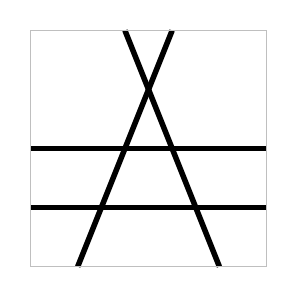
\begin{tikzpicture}[scale=3]
    \draw[line width=2] (0.2,0)--(0.6,1);
    \draw[line width=2] (0.8,0)--(0.4,1);
    \draw[line width=2] (0,0.5)--(1,0.5);
    \draw[line width=2] (0,0.25)--(1,0.25);
    \draw[gray!50] (0,0) rectangle (1, 1);
  \end{tikzpicture}
  ~
  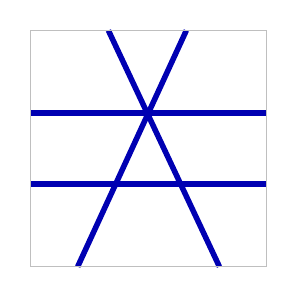
\begin{tikzpicture}[scale=3]
    \draw[blue!70!black, line width=2] (0.2,0)--(0.66,1);
    \draw[blue!70!black, line width=2] (0.8,0)--(0.33,1);
    \draw[blue!70!black, line width=2] (0,0.65)--(1,0.65);
    \draw[blue!70!black, line width=2] (0,0.35)--(1,0.35);
    \draw[gray!50] (0,0) rectangle (1, 1);
  \end{tikzpicture}
  ~
  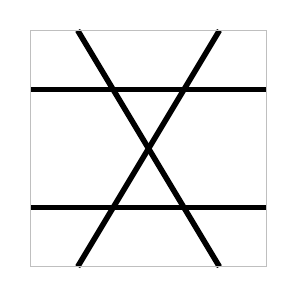
\begin{tikzpicture}[scale=3]
    \draw[line width=2] (0.2,0)--(0.8,1);
    \draw[line width=2] (0.8,0)--(0.2,1);
    \draw[line width=2] (0,0.75)--(1,0.75);
    \draw[line width=2] (0,0.25)--(1,0.25);
    \draw[gray!50] (0,0) rectangle (1, 1);
  \end{tikzpicture}

  \noindent
  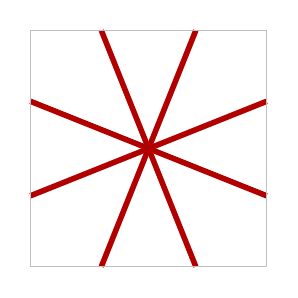
\begin{tikzpicture}[scale=3]
    \draw[red!70!black, line width=2] (0.3,0)--(0.7,1);
    \draw[red!70!black, line width=2] (0.7,0)--(0.3,1);
    \draw[red!70!black, line width=2] (0,0.7)--(1,0.3);
    \draw[red!70!black, line width=2] (0,0.3)--(1,0.7);
    \draw[gray!50] (0,0) rectangle (1, 1);
  \end{tikzpicture}
  ~
  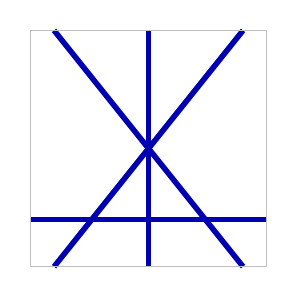
\begin{tikzpicture}[scale=3]
    \draw[blue!70!black, line width=2] (0.1,0)--(0.9,1);
    \draw[blue!70!black, line width=2] (0.9,0)--(0.1,1);
    \draw[blue!70!black, line width=2] (0,0.2)--(1,0.2);
    \draw[blue!70!black, line width=2] (0.5,0)--(0.5,1);
    \draw[gray!50] (0,0) rectangle (1, 1);
  \end{tikzpicture}
  ~
  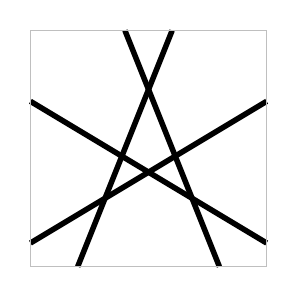
\begin{tikzpicture}[scale=3]
    \draw[line width=2] (0.2,0)--(0.6,1);
    \draw[line width=2] (0.8,0)--(0.4,1);
    \draw[line width=2] (0,0.7)--(1,0.1);
    \draw[line width=2] (0,0.1)--(1,0.7);
    \draw[gray!50] (0,0) rectangle (1, 1);
  \end{tikzpicture}
  \caption{There are $A241600(4) = 9$ arrangements of $4$ lines in the plane,
  which split the plane into $5, 8, 9, 10, 9, 10, 8, 10$, and $11$ parts
  respectively.}
\end{figure}

\begin{question}
  How many nonisomorphic ways can $n$ lines split the plane into $k$ parts?
\end{question}

\begin{related}
  \item What if only two lines can go through a single point?
  \item What if circles are used instead of lines? Circles on a sphere? Lines on a torus?
  \item Hyperplanes in higher dimensional space?
  \item How many arrangements are there if the bounded regions must have equal
    area?
  \item How many different polygons can be embedded such that every side is
    on a line? Convex polygons?
\end{related}

\begin{references}
  \item OEIS sequences
    \href{https://oeis.org/A241600}{A241600},
    \href{https://oeis.org/A177862}{A177862}, and
    \href{https://oeis.org/A250001}{A250001}.
\end{references}
\end{document}
